% Kopfzeile beim Kapitelanfang:
\fancypagestyle{plain}{
%Kopfzeile links bzw. innen
\fancyhead[L]{\Large Vorlesung 9 (11.11.2013)}
%Kopfzeile rechts bzw. außen
\fancyhead[R]{}}
%Kopfzeile links bzw. innen
\fancyhead[L]{\Large Vorlesung 9 (11.11.2013)}
%Kopfzeile rechts bzw. außen
\fancyhead[R]{}
% **************************************************
\subsection*{Beispiel}
$a_n := (-1)^n + \frac{1}{n}$ ist beschränkt, aber nicht konvergent.\\
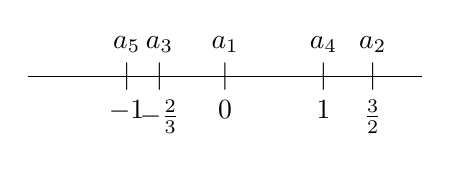
\begin{tikzpicture}
\draw(0,0)--(5,0);
\foreach \x/\xtext/\ytext in {2.5/$0$/$a_1$, 1.25/$-1$/$a_5$, 3.75/$1$/$a_4$, 1.6666666/$-\frac{2}{3}$/$a_3$, 4.375/$\frac{3}{2}$/$a_2$}
  \draw(\x,0pt) node{$|$} (\x,-5pt) node[below] {\xtext} (\x,+5pt) node[above] {\ytext};
\end{tikzpicture}\\
$a_{2n} = 1 + \frac{1}{2n} \to 1$\\
$a_{2n+1} = -1 + \frac{1}{2n+1} \to -1$\\
$(a_{2n})_{n \in \N}$ und $(a_{2n+1})_{n \in \N}$ sind konvergente Teilfolgen

\section{Definition: Cauchyfolge}\label{5.13}
Eine Folge $(a_n)_{n \in \N} \subseteq \R$ heißt \underline{Cauchyfolge} (benannt nach dem französischen Mathematiker \href{https://de.wikipedia.org/wiki/Augustin-Louis_Cauchy}{Augustin-Louis Cauchy}) genau dann, wenn $\forall \eps > 0 \exists n_0 \in \N: |a_n-a_m| < \eps \forall n,m \ge n_0$

\section{Satz: Konvergenz, Cauchyfolge}\label{5.14}
Sei $(a_n) \subseteq \R$ konvergent $\Ra (a_n)$ ist Cauchyfolge.

\subsection*{Beweis}
$a_n \to a \Ra |a_n-a_m| - |a_n-a+a-a_m| \underset{\text{Dreiecksungl.}}{\le} |a_n-a| + |a-a_m|$\\
Wähle $n_0$ so groß, dass $|a_n-a| < \frac{\eps}{2} \forall n \ge n_0$\\
$\Ra \forall n-m \ge n_0: |a_n-a_m| < \frac{\eps}{2} + \frac{\eps}{2} = \eps$ \qed

\section{Satz: Cauchy-Kriterium}\label{5.15}
Jede Cauchyfolge $(a_n) \subseteq \R$ ist konvergent.

\subsection*{Beweis}
$(a_n)$ ist beschränkt, denn $\exists n_0 \in \N: |a_n-a_{n_0}| < 1 \forall n \ge n_0$\\
$\Ra |a_n| \le max\{|a_1|,|a_2|,\hdots,|a_{n_0}|,|a_{n_0}+1|\} < \infty$
Bolzano-Weierstraß $\Ra (a_n)$ hat konvergente Teilfolge $(a_{n_k})_{k \in \N}$\\
$a := \lim_{k \to \infty} a_{n_k}$

\section*{Behauptung}
$(a_n)_{n \in \N}$ konvergiert gegen $a$.

\subsection*{Beweis}
Sei $\eps > 0 \Ra |a_{n_k}-a| < \frac{\eps}{2} \forall k \ge N_1$\\
$|a_n-a_m| < \frac{\eps}{2} \forall n,m \ge N_2$\\
$k \ge max(N_1,N_2) \Ra |a_k-a| \underset{\text{Dreiecksungl.}}{\le} \underbrace{|a_k-a_{n_k}|}_{\text{da } n_k \ge k} + \underbrace{|a_{n_k}-a|}_{< \frac{\eps}{2}} \Ra |a_k-a| < \eps$ \qed

\section{\texorpdfstring{Definition: Uneigentliche Konvergenz gegen $\pm \infty$}{Definition: Uneigentliche Konvergenz gegen \textbackslash{pm} \textbackslash{infty}}}\label{5.16}
$(a_n)_{n \in \N} \subseteq \R$ heißt \underline{uneigentlich konvergent} gegen $+\infty$ \emph{[bzw. gegen $-\infty$]}, falls gilt:\\
$\forall M > 0 \exists n_0 \in \N: a_n > M \forall n \ge n_0$ \emph{[bzw. $a_n < -M \forall n \ge n_0$]}

\subsection*{Schreibweise}
$\lim_{n \to \infty} a_n = +\infty$ \emph{[bzw. $\lim_{n \to \infty} a_n = -\infty$]}

\subsection*{Beispiele}
\en{
\item $\lim_{n \to \infty} n = +\infty$
\item $(a_n)$ sei monoton wachsend und nach oben unbeschränkt.\\
$\Ra \forall M > 0 \exists n_0 \in \N: a_{n_0} > M \underset{\text{Monotonie}}{\Ra} a_n > M \forall n \ge n_0$\\
$\Ra \lim_{n \to \infty} a_n = +\infty$
\item $a_n = (-1)^n \cdot n$ ist weder konvergent, noch uneigentlich konvergent.
}

\section{Lemma}\label{5.17}
$\lim_{n \to \infty} a_n = +\infty \Lra \exists n_0 \in \N: a_n \neq 0 \forall n \ge n_0$ und $\lim_{n \to \infty} \frac{1}{a_n} = 0$\\
Denn: Für $M > 0$ gilt:\\
$a_n > M \forall n \ge n_0 \Lra 0 < \frac{1}{a_n} < \frac{1}{M} \forall n \ge n_0$ \qed

\newpage

\section{Definition: Landau-Symbole}\label{5.18}
Seien $(a_n),(b_n) \subseteq \R$ Folgen. Man schreibt:
\en{
\item $a_n = O(b_n)$ für $n \to \infty$, falls $\exists c > 0$ und $n_0 \in \N: |a_n| \le c|b_n| \forall n \ge n_0$\\
anschaulich: $(a_n)$ wächst höchstens so schnell wie $(b_n)$.
\item $a_n = \Theta(b_n)$ für $n \to \infty$, falls $a_n = O(b_n)$ und $b_n = O(a_n)$, das heißt $(a_n)$ und $(b_n)$ wachsen gleich schnell.
\item $a_n = o(b_n)$ für $n \to \infty$, falls $\lim_{n \to \infty} \frac{a_n}{b_n} = 0$, das heißt $(b_n)$ wächst schneller als $(a_n)$.
}

\subsection*{Beachte}
\enk{
\item Existiert $\lim_{n \to \infty} \frac{a_n}{b_n} =: c \in \R \Ra a_n = O(b_n)$ (Übung)
\item $a_n = o(b_n) \Ra a_n = O(b_n)$
}

\subsection*{Beispiele}
\enk{
\item $a_n = 2n^2 - 5 \Ra a_n = O(n^2)$, da $\lim_{n \to \infty} \frac{a_n}{n_2} = 2$\\
sogar $a_n = \Theta(n^2)$ (da $\lim_{n \to \infty} \frac{n^2}{a_n} = \frac{1}{2}$)\\
Dagegen \underline{nicht}: $a_n = O(n)$, da $\frac{a_n}{n} = 2n - \frac{5}{n}$ unbeschränkt.\\
$a_n = o(n^3)$, da $\lim_{n \to \infty} \frac{a_n}{n^3} = 0$
\item $a_n$ sei die Zahl der Rechenoperationen, die ein Computer benötigt, um eine Liste der Länge $n$ mit \href{https://de.wikipedia.org/wiki/Bubblesort}{Bubblesort} zu sortieren: $a_n=O(n^2)$\\
Mit \href{https://de.wikipedia.org/wiki/Quicksort}{Quicksort}: $O(n \log n)$
}

\chapter{Komplexe Zahlen}\label{P6}
\section*{Motivation}
Die Gleichung (*) $x^2+1=0$ hat keine Lösung im $\R$,\\
denn: $x \in \R \underset{Anordnungsax.}{\Ra} x^2 > 0 \Ra x^2 + 1 > 0$

\subsection*{Ziel}
Konstruktion eines Körpers $\C$, der $\R$ umfasst und in dem (*) lösbar ist.

\section*{Vorüberlegung}
Angenommen, es existiert ein Körper $\C$ mit $\R \subseteq \C$,\\
so dass (*) eine Lösung $i \in \C$ hat ($i$ wie \emph{``imaginär''})

\subsection*{Rechenregeln}
Für $\Ra x,y,z,v \in \R$ gilt:
\items{
\item $(x+iy)+(u+iv)=(x+u)+i(y+v)$
\item $(x+iy)\cdot(u+iv)=xu + i^2 yv + i(xv+yu) = xu-yv+i(xv+yu)$
}

\section{Definition: Rechnen mit komplexen Zahlen}\label{6.1}
Gegeben sei $\C := \R \times \R$ mit\\
Addition: $(x,y)+(u,v) := (x+u,y+v)$\\
Multiplikation: $(x,y)\cdot(u,v) := (xu-yv,xv+yu)$

\section{Satz: Körper der komplexen Zahlen}\label{6.2}
$(\C, +, \cdot)$ ist der \underline{Körper der komplexen Zahlen}.

\subsection*{Beweis}
$+, \cdot$ sind kommutativ, $+$ assoziativ und das Distributivgesetz ist erfüllt (leicht nachzurechnen).\nl
Neutrale Elemente:\\
bzgl. $+$ : $0 = (0,0)$\\
bzgl. $\cdot$ : $1 = (1,0)$\nl
Inverse: $-(x,y)=(-x,-y)$\\
$(x,y) \neq (0,0) \Ra (x,y)^{-1} = \bigbrackets{\frac{x}{x^2+y^2}, \frac{-y}{x^2+y^2}}$

\newpage

\section*{$\R$ als Teilkörper von $\C$}
$(x,0) \dotplus (y,0) = (x \dotplus y, 0)$ \emph{($\dotplus$ steht für: ``mal/plus'', ähnlich wie $\pm$)}\\
Man identifiziert daher $x \in \R$ mit $(x,0) \in \C$ und fasst $\R$ als Teilkörper von $\C$ auf.

\subsection*{Bezeichnung}
$i := (0,1) \in \C$ ist die \underline{imaginäre Einheit}.
Damit: $i^2 = (0,1) \cdot (0,1) = (-1,0) = -1$\\
$\Ra i$ und $-i = (-1) \cdot i$ lösen die Gleichung $x^2+1=0$.\nl
Ferner: $\C \ni z = (x,y) \Lra z = (x,0)+(0,y) = (x,0)+(0,1) \cdot (y,0) \Lra y=x+iy$\\
Jedes $z \in \C$ hat daher eine eindeutige Darstellung der Form $z = x+iy$ mit $x,y \in \R$.

\section{Definition: Realteil, Imaginärteil}\label{6.3}
Sei $z = x+iy \in \C$ ($x,y \in \R$). Dann sind\\$\text{Re } z := x$ der \underline{Realteil} von $z$ und\\
$\text{Im } z := y$ der \underline{Imaginärteil} von $z$.\nl
$z$ heißt \underline{reell}, falls $\text{Im } z = 0$, $z$ heißt \underline{imaginär}, falls $\text{Re } z = 0$.

\subsection*{Geometrische Veranschaulichung der komplexen Zahlenebene}\label{GeoKompZE}
(nach \href{https://de.wikipedia.org/wiki/Carl_Friedrich_Gau\%C3\%9F}{Carl Friedrich Gauß}, um 1800)\\
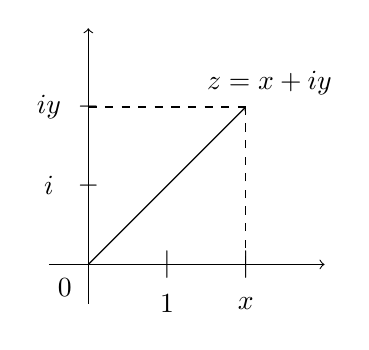
\begin{tikzpicture}
\draw[->](-0.5,0)--(3,0);
\draw[->](0,-0.5)--(0,3);
\draw (-0.3,-0.3) node{$0$};
\draw (1,0) node{$|$};
\draw (1,-0.5) node{$1$};
\draw (2,0) node{$|$};
\draw (2,-0.5) node{$x$};
\draw (0,1) node{$-$};
\draw (-0.5,1) node{$i$};
\draw (0,2) node{$-$};
\draw (-0.5,2) node{$iy$};
\draw[->](0,0)--(2,2);
\draw[dashed](0,2)--(2,2);
\draw[dashed](2,0)--(2,2);
\draw (2.3,2.3) node{$z=x+iy$};
\end{tikzpicture}

\newpage

\section{Definition: Komplexe Konjugation und Betrag}\label{6.4}
Sei $z = x+iy \in \C$ ($x,y \in \R$).\\
$\overline{z} := x-iy$ \underline{konjugiert komplexe Zahl}

\subsection*{Geometrisch}
$z \mto \overline{z}$ ist Spiegelung an der reellen Achse.\\
\begin{tikzpicture}
\draw[->](-1,0)--(3,0);
\draw[->](0,-3)--(0,3);
\draw (-0.3,-0.3) node{$0$};
\draw (0,2) node{$-$};
\draw (-0.5,2) node{$iy$};
\draw (0,-2) node{$-$};
\draw (-0.5,-2) node{$-iy$};
\draw[->](0,0)--(2,2);
\draw[->](0,0)--(2,-2);
\draw[dashed](0,2)--(2,2);
\draw[dashed](2,0)--(2,2);
\draw[dashed](0,-2)--(2,-2);
\draw[dashed](2,0)--(2,-2);
\draw (2.3,2.3) node{$z$};
\draw (2.3,-2.3) node{$\overline{z}$};
\end{tikzpicture}

\section{\texorpdfstring{Eigenschaften von $z \mto \overline{z}$}{Eigenschaften von \mathtt{z} \textbackslash{mto} \textbackslash{overline} \mathtt{z}}}\label{6.5}
\enk{
\item $\overline{\overline{z}} = z$
\item $\overline{z+w} = \overline{z} + \overline{w}$
\item $\overline{zw} = \overline{z} \cdot \overline{w}$
\item $z + \overline{z} = 2 \text{ Re } z, z - \overline{z} = 2 \text{ Im } z$
\item $z = \overline{z} \Lra z \in \R$
\item $z = x+iy (x,y) \Ra z \overline{z} = (x+iy)(x-iy) = x^2-i^2 y^2 = x^2 + y^2 \Ra z \overline{z} \in \R_{+} = [0,\infty)$
}

\subsection*{Beweise}
Bis auf 3. alle klar.\\
Zu 3.: $z = x+iy, w=u+iv \Ra \overline{zw} = \overline{(x+iy)(u+iv)} = \overline{xu-yv+i(yu+xv)} = xu-yv-i(yu+xv)=(x-iy)(u-iv)$ \ok